\documentclass{ximera}

\title{Multivariable Optimization: Second Derivatives}
\author{Zack Reed}

\begin{document}
\begin{abstract}
In this activity we explore quadratic approximations of functions of multiple variables, introducing the Hessian matrix and the second derivative test for classifying critical points.
\end{abstract}
\maketitle


\section*{Quadratic Approximations of Functions: The Hessian Matrix and the Second Derivative Test}

Just as $f^{\prime\prime}(x)$ tells us about concavity in single-variable calculus, the \textbf{Hessian matrix} captures second-order information in multiple variables. 

While we'll gloss over some details, the important takeaway is that from the Hessian matrix we build a quadratic approximation of the function at a point, just like the 2nd degree Taylor polynomial in single-variable calculus.

\subsection*{Defining the Hessian}

\begin{definition}
For a function $f(x,y)$, the \textbf{Hessian matrix} is:
$$H = \begin{bmatrix}
\frac{\partial^2 f}{\partial x^2} & \frac{\partial^2 f}{\partial x \partial y} \\
\frac{\partial^2 f}{\partial y \partial x} & \frac{\partial^2 f}{\partial y^2}
\end{bmatrix}$$

The entries are:
\begin{itemize}
    \item $\frac{\partial^2 f}{\partial x^2}$: second partial derivative with respect to $x$
    \item $\frac{\partial^2 f}{\partial y^2}$: second partial derivative with respect to $y$
    \item $\frac{\partial^2 f}{\partial x \partial y}$ and $\frac{\partial^2 f}{\partial y \partial x}$: mixed partial derivatives (usually equal)
\end{itemize}
\end{definition}

\begin{problem}
Let's compute the Hessian of $f(x,y) = x^2 + y^2$.

First derivatives: $\frac{\partial f}{\partial x} = 2x$ and $\frac{\partial f}{\partial y} = 2y$

Second derivatives:
$$\frac{\partial^2 f}{\partial x^2} = \frac{\partial}{\partial x}(2x) = \answer{2}$$
$$\frac{\partial^2 f}{\partial y^2} = \frac{\partial}{\partial y}(2y) = \answer{2}$$
$$\frac{\partial^2 f}{\partial x \partial y} = \frac{\partial}{\partial y}(2x) = \answer{0}$$

The Hessian matrix is:
$$H = \begin{bmatrix} \answer{2} & \answer{0} \\ \answer{0} & \answer{2} \end{bmatrix}$$


Notice that this Hessian is constant - it doesn't depend on $(x,y)$! This mirrors the properties of quadratic functions in single-variable calculus, where the second derivative is constant.
\end{problem}

\begin{problem}
Compute the Hessian of $f(x,y) = x^3 + y^3 - 3xy$.

First derivatives: $\frac{\partial f}{\partial x} = 3x^2 - 3y$ and $\frac{\partial f}{\partial y} = 3y^2 - 3x$

Second derivatives:
$$\frac{\partial^2 f}{\partial x^2} = \answer{6x}$$
$$\frac{\partial^2 f}{\partial y^2} = \answer{6y}$$
$$\frac{\partial^2 f}{\partial x \partial y} = \answer{-3}$$

The Hessian matrix is:
$$H = \begin{bmatrix} \answer{6x} & \answer{-3} \\ \answer{-3} & \answer{6y} \end{bmatrix}$$

Now, the second derivatives change according to the location of the point $(x,y)$.

Let's see what the Hessian is at different points:

\begin{enumerate}
    \item At the point $(0,0)$, we have:
    $$H(0,0) = \begin{bmatrix} \answer{0} & \answer{-3} \\ \answer{-3} & \answer{0} \end{bmatrix}$$

    \item At the point $(1,1)$, we have:
    $$H(1,1) = \begin{bmatrix} \answer{6} & \answer{-3} \\ \answer{-3} & \answer{6} \end{bmatrix}$$

    \item At the poitn $(1,-1)$, we have:
    $$H(1,-1) = \begin{bmatrix} \answer{6} & \answer{-3} \\ \answer{-3} & \answer{-6} \end{bmatrix}$$
\end{enumerate}
\end{problem}

\section*{Quadratic Approximations}

Much like quadratic Taylor approximations in single-variable calculus, we can use the Hessian to build a quadratic approximation of a multivariable function at a point.

\begin{definition}
The \textbf{quadratic approximation} of $f(x,y)$ at the point $(x_0, y_0)$ is:
\begin{align*}
Q(x,y) = & f(x_0, y_0) + \frac{\partial f}{\partial x}(x - x_0) + \frac{\partial f}{\partial y}(y - y_0) \\
& + \frac{1}{2} \left(\frac{\partial^2 f}{\partial x^2}(x - x_0)^2 + 2\frac{\partial^2 f}{\partial x \partial y}(x - x_0)(y - y_0) + \frac{\partial^2 f}{\partial y^2}(y - y_0)^2 \right)
\end{align*}

Here, all of the derivatives are calculated at the point $(x_0, y_0)$.
\end{definition}


In single-variable calculus, we had three standard cases for classifying critical points using the second derivative: 
\begin{itemize}
    \item If $f^{\prime\prime}(x_0) > 0$, local minimum
    \item If $f^{\prime\prime}(x_0) < 0$, local maximum
    \item If $f^{\prime\prime}(x_0) = 0$, test is inconclusive
\end{itemize}

This idea came from quadratic approximation. Quadratic functions either open up, open down, or are flat.

In multiple variables, quadratic surfaces can take on three forms instead of two:

%list out and visualize each case with an actual quadratic formula for the surface
\begin{itemize}
    \item Bowl-shaped (local min or max)
    
    The following quadratic surface is $f(x,y) = x^2 + y^2$, which has a local minimum at the origin. Quadratic approximations behaving like this indicate local minima (and their negatives indicate local maxima).
    
    \begin{center}
    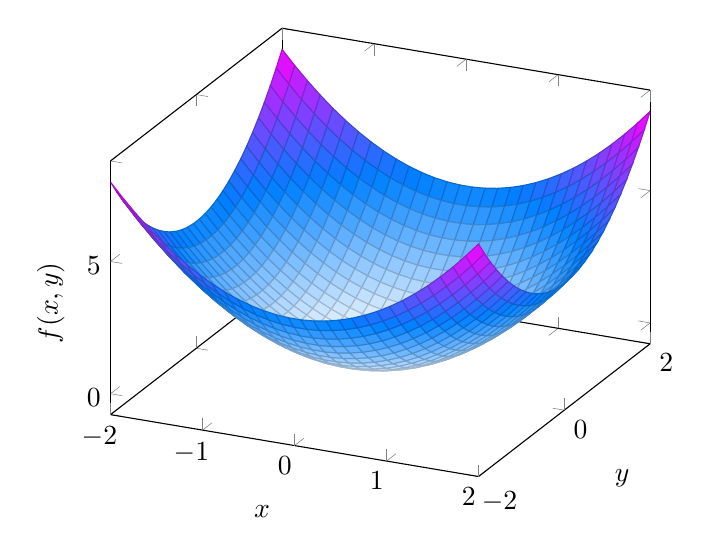
\begin{tikzpicture}
        \begin{axis}[
            domain=-2:2,
            samples=30,
            xlabel=$x$,
            ylabel=$y$,
            zlabel={$f(x,y)$},
            colormap/cool,
            ]
            \addplot3[surf] {x^2 + y^2};
        \end{axis}
    \end{tikzpicture}
    \end{center}

    \item Saddle-shaped (saddle point)
    
    The following quadratic surface is $f(x,y) = x^2 - y^2$, which has a saddle point at the origin. Quadratic approximations behaving like this indicate saddle points.
    \begin{center}
    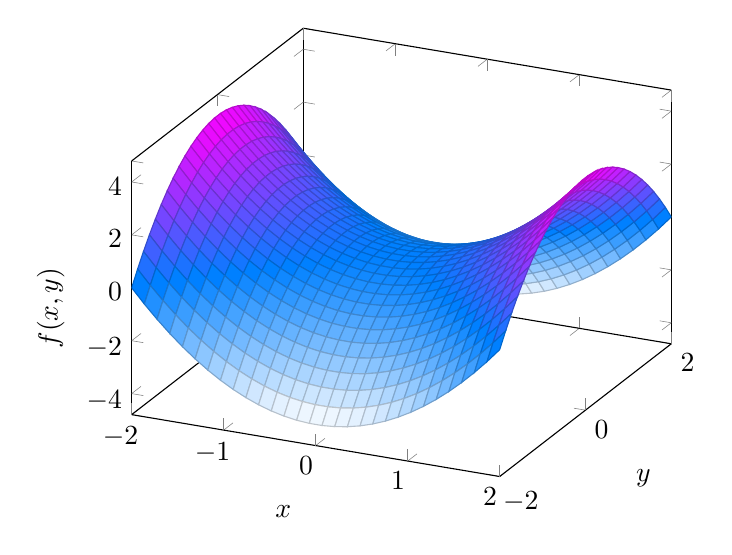
\begin{tikzpicture}
        \begin{axis}[
            domain=-2:2,
            samples=30,
            xlabel=$x$,
            ylabel=$y$,
            zlabel={$f(x,y)$},
            colormap/cool,
            ]
            \addplot3[surf] {x^2 - y^2};
        \end{axis}
    \end{tikzpicture}
    \end{center}

    \item Flat or complex (test inconclusive)
    
    The following quadratic surface is $f(x,y) = x^3 - y^3$, which has a flat region at the origin. Quadratic approximations behaving like this indicate that the second derivative test is inconclusive.
    \begin{center}
    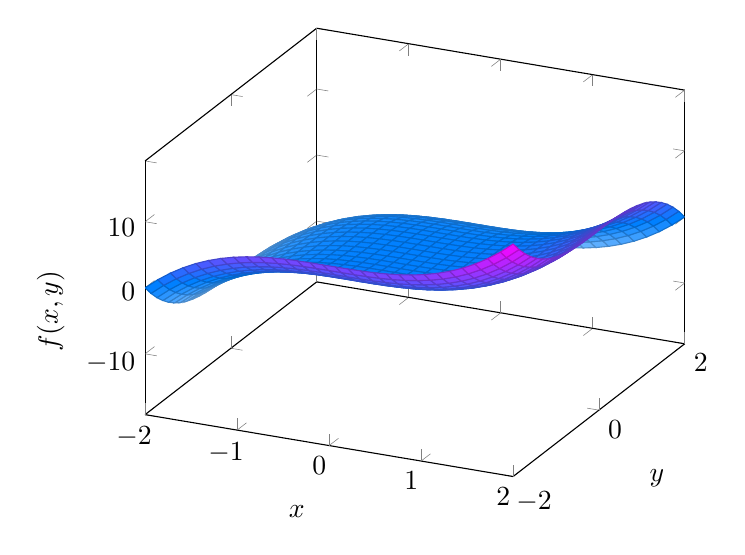
\begin{tikzpicture}
        \begin{axis}[
            domain=-2:2,
            samples=30,
            xlabel=$x$,
            ylabel=$y$,
            zlabel={$f(x,y)$},
            colormap/cool,
            ]
            \addplot3[surf] {x^3 - y^3};
        \end{axis}
    \end{tikzpicture}
    \end{center}
\end{itemize}



\subsection*{The Second Derivative Test}

Much like how we only needed to know the sign of the second derivative in single-variable calculus, we can classify critical points in multiple variables using just a couple values from the Hessian matrix.

We use a pseudo-equivalent to looking at the sign, taking what is called the \emph{determinant} of the Hessian.

\begin{definition}
Let $(x_0, y_0)$ be a critical point and let $H$ be the Hessian evaluated at that point. Define:

$$D = \det(H) = \frac{\partial^2 f}{\partial x^2} \frac{\partial^2 f}{\partial y^2} - \left(\frac{\partial^2 f}{\partial x \partial y}\right)^2$$ 

to be the \emph{determinant} of the Hessian matrix at $(x_0, y_0)$. In typical multivariable calculus textbooks this is called the \emph{descriminant}, but we find it important to make connections when we can, so we're going to describe this in terms of determinants, which come up in later courses.

Then:
\begin{itemize}
    \item If $D > 0$ and $\frac{\partial^2 f}{\partial x^2} > 0$: \textbf{local minimum}
    \item If $D > 0$ and $\frac{\partial^2 f}{\partial x^2} < 0$: \textbf{local maximum}
    \item If $D < 0$: \textbf{saddle point}
    \item If $D = 0$: \textbf{test is inconclusive}
\end{itemize}
\end{definition}


The following video visualizes the process of quadratic approximation, the finding of the Hessian, and the second derivative test.

\begin{center}
\youtube{PTrbdL7Pkiw}
\end{center}

Let's practice using the second derivative test on a few cases that we've already seen.

\begin{problem}
Why does the sign of $\frac{\partial^2 f}{\partial x^2}$ matter when $D > 0$?

\begin{multipleChoice}
    \choice{It determines whether the function is differentiable}
    \choice[correct]{It tells us the concavity in the $x$-direction}
    \choice{It measures the steepness of the gradient}
    \choice{It doesn't actually matter}
\end{multipleChoice}

\end{problem}

\begin{problem}
Let's classify the critical point of $f(x,y) = x^2 + y^2 - 4x + 6y + 5$ at $(2, -3)$.

\begin{center}
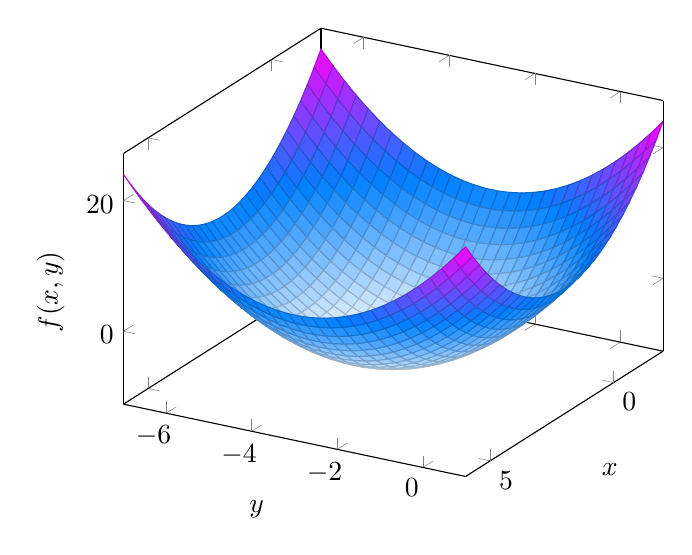
\begin{tikzpicture}
    \begin{axis}[
        domain=-2:6,
        y domain=-7:1,
        samples=30,
        xlabel=$x$,
        ylabel=$y$,
        zlabel={$f(x,y)$},
        colormap/cool,
        view={120}{30},
        ]
        \addplot3[surf] {x^2 + y^2 - 4*x + 6*y + 5};
    \end{axis}
\end{tikzpicture}
\end{center}

We found earlier that the Hessian is:
$$H = \begin{bmatrix} 2 & 0 \\ 0 & 2 \end{bmatrix}$$

The discriminant is:
$$D = (2)(2) - (0)^2 = \answer{4}$$

Since $D > 0$ and $\frac{\partial^2 f}{\partial x^2} = 2 > 0$, the critical point is a \wordChoice{\choice[correct]{local minimum}\choice{local maximum}\choice{saddle point}}.

The minimum value is:
$$f(2,-3) = 4 + 9 - 8 - 18 + 5 = \answer{-8}$$

\begin{feedback}
    This makes sense - the function is $(x-2)^2 + (y+3)^2 - 8$, a paraboloid with vertex at $(2,-3,-8)$.
\end{feedback}
\end{problem}

\begin{problem}
Classify the critical point of $f(x,y) = x^2 - y^2$ at $(0,0)$.

\begin{center}
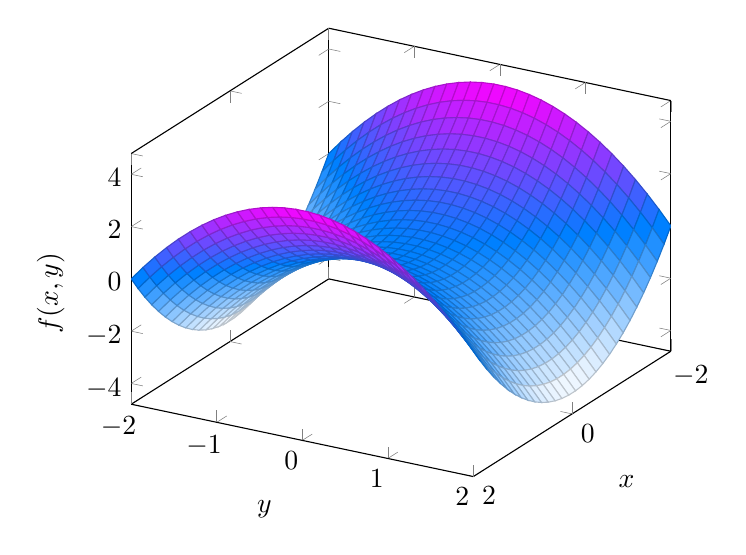
\begin{tikzpicture}
    \begin{axis}[
        domain=-2:2,
        samples=30,
        xlabel=$x$,
        ylabel=$y$,
        zlabel={$f(x,y)$},
        colormap/cool,
        view={120}{30},
        ]
        \addplot3[surf] {x^2 - y^2};
    \end{axis}
\end{tikzpicture}
\end{center}

The Hessian is:
$$H = \begin{bmatrix} 2 & 0 \\ 0 & -2 \end{bmatrix}$$

The discriminant is:
$$D = (2)(-2) - (0)^2 = \answer{-4}$$

Since $D < 0$, the critical point is a \wordChoice{\choice{local minimum}\choice{local maximum}\choice[correct]{saddle point}}.

\begin{feedback}
    When $D < 0$,the function curves up in one direction and down in another, creating a saddle shape.
\end{feedback}
\end{problem}

\begin{problem}
Now a complete example. Find and classify all critical points of:
$$f(x,y) = x^3 + y^3 - 3xy$$

\begin{center}
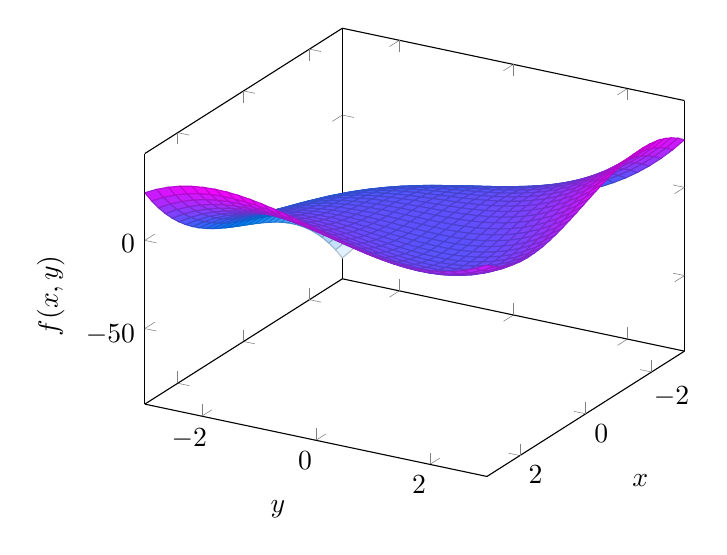
\begin{tikzpicture}
    \begin{axis}[
        domain=-3:3,
        samples=30,
        xlabel=$x$,
        ylabel=$y$,
        zlabel={$f(x,y)$},
        colormap/cool,
        view={120}{30},
        ]
        \addplot3[surf] {x^3 + y^3 - 3*x*y};
    \end{axis}
\end{tikzpicture}
\end{center}

\textbf{Step 1: Find critical points}

The gradient is $\nabla f = \langle 3x^2 - 3y, 3y^2 - 3x \rangle$

Setting both components to zero:
$$x^2 - y = 0 \Rightarrow y = x^2$$
$$y^2 - x = 0 \Rightarrow y^2 = x$$

Substituting: $(x^2)^2 = x \Rightarrow x^4 - x = 0 \Rightarrow x(x^3-1) = 0$

So $x = \answer{0}$ or $x = \answer{1}$ (put the smaller number first)

The critical points are: $(\answer{0}, \answer{0})$ and $(\answer{1}, \answer{1})$.


\textbf{Step 2: Compute the Hessian}

$$H = \begin{bmatrix} 6x & -3 \\ -3 & 6y \end{bmatrix}$$

\textbf{Step 3: Classify $(0,0)$}

$$H(0,0) = \begin{bmatrix} 0 & -3 \\ -3 & 0 \end{bmatrix}$$

$$D = (0)(0) - (-3)^2 = \answer{-9}$$

Since $D < 0$, $(0,0)$ is a \wordChoice{\choice{local minimum}\choice{local maximum}\choice[correct]{saddle point}}.

% %show the same surface but with a quadratic approximation at (0,0) to visualize the saddle shape
% \begin{center}
% \begin{tikzpicture}
%     \begin{axis}[
%         domain=-3:3,
%         samples=30,
%         xlabel=$x$,
%         ylabel=$y$,
%         zlabel={$f(x,y)$},
%         colormap/cool,
%         view={120}{30},
%         ]
%             % \addplot3[surf] {x^3 + y^3 - 3*x*y};
%         \addplot3[surf, opacity=0.5] {0 -3*x*y};
%     \end{axis}
% \end{tikzpicture}
% \end{center}


\textbf{Step 4: Classify $(1,1)$}

$$H(1,1) = \begin{bmatrix} 6 & -3 \\ -3 & 6 \end{bmatrix}$$

$$D = (6)(6) - (-3)^2 = 36 - 9 = \answer{27}$$

Since $D > 0$ and $\frac{\partial^2 f}{\partial x^2} = 6 > 0$, $(1,1)$ is a \wordChoice{\choice[correct]{local minimum}\choice{local maximum}\choice{saddle point}}.

The extreme value is: $f(1,1) = 1 + 1 - 3 = \answer{-1}$

% %show the same surface but with a quadratic approximation at (1,1) to visualize the bowl shape
% \begin{center}
% \begin{tikzpicture}
%     \begin{axis}[
%         domain=-3:3,
%         samples=30,
%         xlabel=$x$,
%         ylabel=$y$,
%         zlabel={$f(x,y)$},
%         colormap/cool,
%         view={120}{30},
%         ]
%         % \addplot3[surf] {x^3 + y^3 - 3*x*y};
%         %quadratic approximation from hessian values
%         \addplot3[surf, opacity=0.5] {1 -3*(x-1)-3*(y-1)+.5*(6*(x-1)^2 - 6*(x-1)*(y-1) + 6*(y-1)^2)};
%     \end{axis}
% \end{tikzpicture}
% \end{center}

\begin{feedback}
    This function has both a saddle point and a local minimum! Real-world optimization problems often have complex landscapes with multiple critical points.
\end{feedback}
\end{problem}

\end{document}
